\chapter{Experiments}

\section{Synthetic data}

The experiments that follow use synthetic data generated from a structural causal model, which is shown in Figure \ref{fig:scm}.

\begin{figure}[!htb]
	\centering
	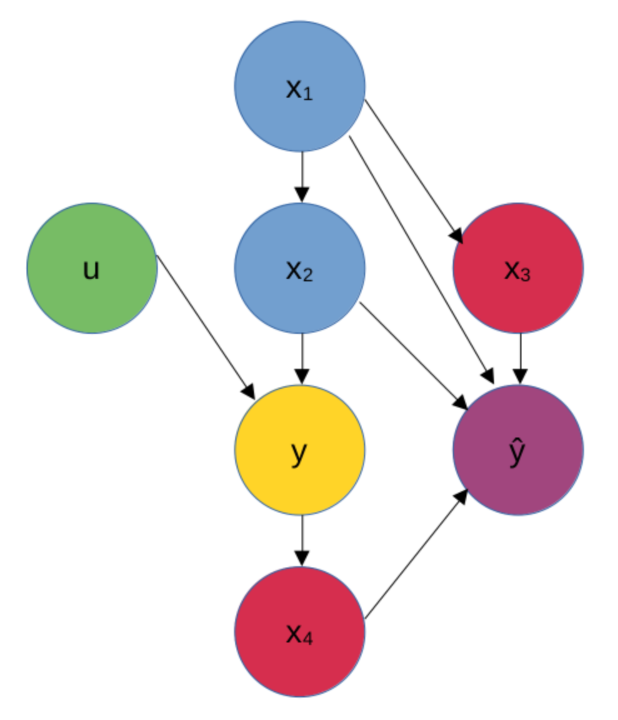
\includegraphics[width=0.4\linewidth]{images/scm.png}
	\caption{The Structural Causal Model used for synthetic data generation}
	\label{fig:scm}
\end{figure}

The structural causal model contains 2 unobserved variables
\begin{itemize}
	\item $\mathbf{u}$ - which is sampled from a normal distribution
	\item $\mathbf{y}$ - the true binary outcome which is a linear combination of $\mathbf{u}$ and $\mathbf{x}_2$
\end{itemize}

And 4 observed variables
\begin{itemize}
	\item $\mathbf{x}_1$ - which is sampled from a normal distribution
	\item $\mathbf{x}_2,\mathbf{x}_3,\mathbf{x}_4$ - which are linear combinations of other variables
	\item $\hat{\mathbf{y}}$ - The predicted value of $\mathbf{y}$
\end{itemize}


\section{Simulation process}

[\textbf{TO CONVERT TO AN ALGORITHM/PSEUDOCODE}]

The process for simulation is as follows. We assume that the individuals do \textit{not} have any knowledge of the classifier.

1. Split the data into test and train sets.

2. Fit a classifier using just the train set and measure accuracy against the *true* labels.

3. Predict labels for \textit{all} data points (both train and test)

4. Calculate recourse actions for all negatively classified data points, by minimising the current approximation of the cost function.

5. Perturb the recourse actions to create pairwise comparisons for the negatively classified individuals to evaluate.

6. Learn cost function from evaluated pairwise comparisons from \textit{all} previous iterations.

7. Generate updated recourse with the current approximation of the cost function.

8. For individuals with a ground truth cost smaller than the cost threshold B, they modify their features to those suggested by recourse. If the ground truth cost of recourse is greater than C, we assume no action is taken.

9. Update the predicted and true labels using the structural causal model (not all instances that involve recourse lead to a change in the true label).

10. Repeat steps 2-9 for a set number of iterations, keeping the same individuals in the train/test sets.

\section{Mahalanobis distance}

Figure \ref{fig:mahanalobis_learning} shows the cumulative proportion of individuals who were negatively classified and have been offered recourse packages with a ground truth cost $c^G(\textbf{x, x'})<B$. If the approximated cost function $c(\textbf{x,x'})$ is close to the ground truth, the recourse suggestions will be closer to the optimal recourse. If the approximated cost is not similar to the ground truth cost function, the recourse suggestions will be further from the optimal recourse and it will be less likely that an individual is successfully offered recourse. The learned cost function outperforms the quadratic and other Mahalanobis cost functions. Figure \ref{fig:mahanalobis_learning} has an assumed ground truth cost function which takes a Mahalanobis form, with a randomly sampled $\textbf{M}$. Additionally, it is assumed that this ground truth function is the same for all individuals.

The next steps to improve this are:
\begin{itemize}
	\item Design a better method for generating the pairwise comparisons (perhaps look into techniques akin to Bayesian Optimisation).
	\item Introduce different ground truth cost functions.
	\item Consider \textit{drift} - where features change over time independently from loan application.
\end{itemize}

\begin{figure}[!htb]
	\centering
	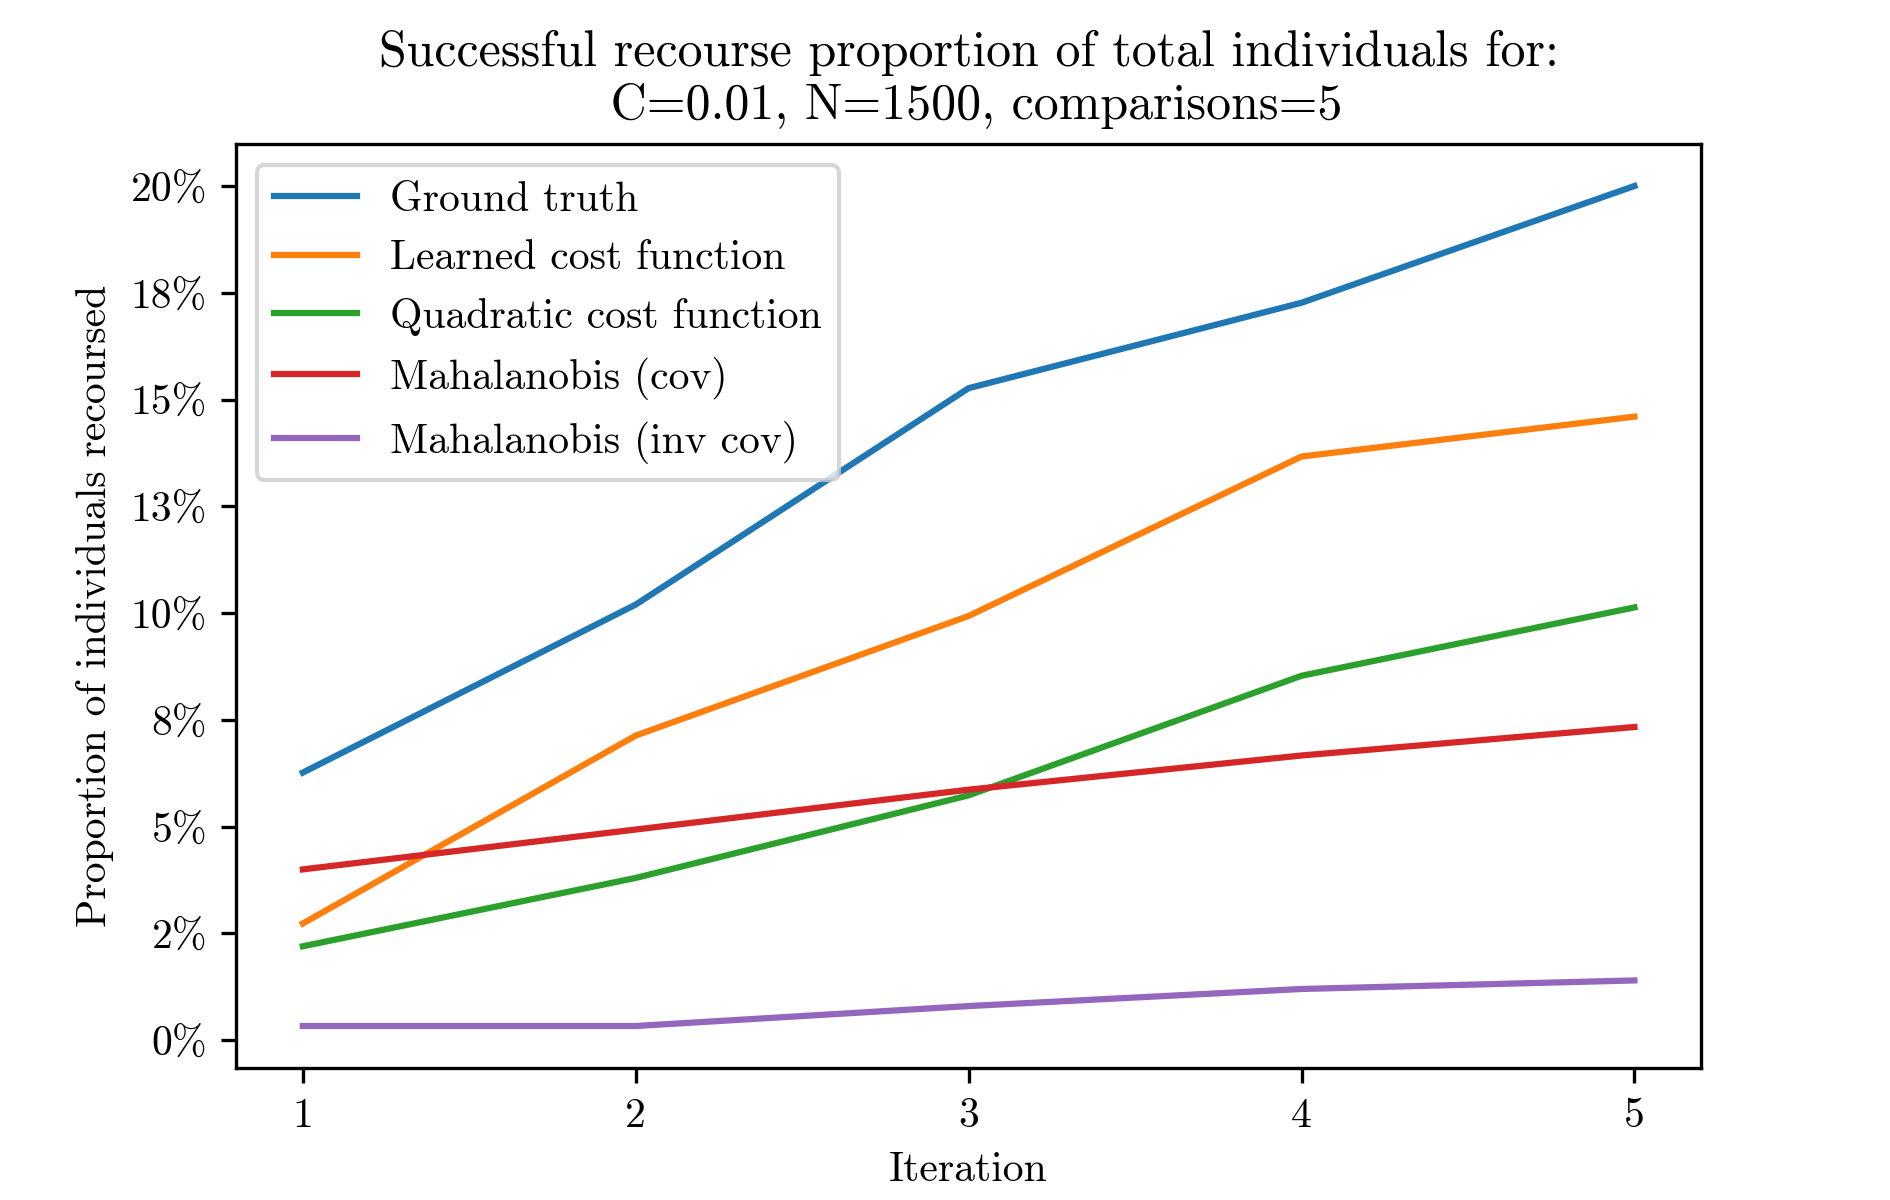
\includegraphics[scale=1]{images/recourse_comparison.png}
	\caption{Cumulative proportion of individuals successfully offered recourse}
	\label{fig:mahanalobis_learning}
\end{figure}